\chapter{Algorithms}

An algorithm here refers to a process or set of processes and calculations
or other problem-solving operations that are performed by a computer.
Algorithms are the most important part of NeTS,
and any other network science library.
They are useful for demonstrating and understanding
fundamental aspects of networks.
As we will see, they can express how connected
a social network is, or even show a profitable exchange path
in a given market.
In this chapter, we will look at functions that
perform algorithms to calculate various values
or to find particular structures in the network.

\section{Neighborhood}
A vertex $x$'s neighborhood $H(x)$ is defined as the set of vertices that are connected to that vertex
by an edge.
In a social network, the neighborhood of a vertex represents
the immediate connections of a user.
In a network that represents the global exchange market for
commodities, the neighborhood can be used to represent
the trade partners of a given country.
The \mintinline{ts}{Network.neighbors(id)}
function returns a list with the IDs of the neighbors of the vertex given.

\begin{minted}[bgcolor=bg]{ts}
neighbors(id: base_id): base_id[] {
  const neighborhood: base_id[] = [];

  this.edges.forEach(({ vertices }) => {
    const { from, to } = vertices;
    if (from === id) neighborhood.push(to);
    else if (to === id) neighborhood.push(from);
  });

  return neighborhood;
}
\end{minted}

This function goes through the Map of edges,
and finds any edge that has one of its vertices match the parameter ID.

When a network is directed, an edge can have two distinct types of neighbors.
In-neighbors are vertices that connect to a vertex $a$ with an edge that ends on $a$.
In other words, for a vertex $a$ in an edge from $b$ to $a$, $b$ is an in-neighbor of $a$.
Out-neighbors are the opposite.

The \mintinline{ts}{inNeighbors} and \mintinline{ts}{outNeighbors} functions
work in a similar fashion to the \mintinline{ts}{neighbors} function.
The difference being that they return a list with neighbors that fulfill
particular properties.

\begin{minted}[bgcolor=bg]{ts}
inNeighbors(id: base_id): base_id[] {
  const in_neighbors: base_id[] = [];
  if (!this.is_directed) return in_neighbors;

  this.edges.forEach(({ vertices }) => {
    const { from, to } = vertices;
    if (to === id) in_neighbors.push(from);
  });

  return in_neighbors;
}

outNeighbors(id: base_id): base_id[] {
  const out_neighbors: base_id[] = [];
  if (!this.is_directed) return out_neighbors;

  this.edges.forEach(({ vertices }) => {
    const { from, to } = vertices;
    if (from === id) out_neighbors.push(to);
  });

  return out_neighbors;
}
\end{minted}

\section{Degree}

The degree of a vertex can be defined as the number of edges that contain said vertex.
Let $E_x$ denote the set of edges containing a vertex $x$, and $D_x$ denote
the degree of $x$. Then,

$$E_x=\{k \mid k \in E, x \in k\}$$
$$D_x=|E_x|$$

The degree of a vertex is, in other words, the number of neighbors for said vertex.
In the example of a social network, the degree of a user would
tells us how many connections that user has in the network.

In this section, we explain the functions related to degree and average degree
for undirected and directed networks.

For an undirected network:

\begin{minted}[bgcolor=bg]{ts}
degree(id: base_id): number {
  let vertex_degree = 0;

  this.edges.forEach(({ vertices }) => {
    const { from, to } = vertices;
    if (from === id || to === id) vertex_degree++;
  });

  return vertex_degree;
}
\end{minted}

The two other degree functions in NeTS are related to in and out-neighbors,
and are only defined when a network is directed.
The function \mintinline{ts}{inDegree} returns the number of edges that end on the given edge.
\mintinline{ts}{outDegree} does the opposite,
returning the number of edges that start on the given vertex.

For a directed network that represents global debt,
let vertices represent countries or international organizations
and edges be directed from borrower to lender.
We could predict that the IMF, for example, has a high out-degree,
as it is a money lender for many countries.
Countries with high in-degree would be those with many debts to pay.

\begin{minted}[bgcolor=bg]{ts}
inDegree(id: base_id): number {
  let in_degree = 0;
  if (!this.is_directed) return in_degree;

  this.edges.forEach(({ vertices }) => {
    const { to } = vertices;
    if (to === id) in_degree++;
  });

  return in_degree;
}

outDegree(id: base_id): number {
  let out_degree = 0;
  if (!this.is_directed) return out_degree;

  this.edges.forEach(({ vertices }) => {
    const { from } = vertices;
    if (from === id) out_degree++;
  });

  return out_degree;
}
\end{minted}

The average degree of a vertex is defined as the sum all its neighbor's degrees over its own degree.
For a vertex $x$, it is usually written as:

$$k_{nn}(x)=\frac{\sum{a_{ix}D(i)}}{D(x)}$$

Where $i$ represents a vertex in the network
and the sum is performed over all vertices in the network.
$a_{ix}$ is $1$ if there is and edge between vertices $i$ and $x$ and $0$ oterwise.
And this is what this would look like when literally transcribed into code:

\begin{minted}[bgcolor=bg]{ts}
averageDegree(id: base_id): number {
  let neighbor_degree_sum = 0;

  this.vertices.forEach(({ id:check_v }) => {
    if (this.hasEdge(id,check_v)) neighbor_degree_sum += this.degree(to);
  });

  return neighbor_degree_sum / this.degree(id);
}
\end{minted}

However, as previously mentioned, we already have a function for getting the neighbors of
a specific vertex.
Thus, we could write the average degree $A_x$ of vertex $x$ as:

$$A_x=\frac{\sum{D(i)}, i\in H(x)}{D(x)}$$

In code:

\begin{minted}[bgcolor=bg]{ts}
averageDegree(id: base_id): number {
  let neighbor_degree_sum = 0;

  this.neighbors(id).forEach((neighbor_id) => {
    neighbor_degree_sum += this.degree(neighbor_id);
  });

  return neighbor_degree_sum / this.degree(id);
}
\end{minted}

This makes it clearer what the \mintinline{ts}{averageDegree} function is supposed to do.
If someone who doesn't know what an average degree is were to look at the assortativity function,
they would have an easier time figuring out what it means.
This is also faster to compute, as we don't need to iterate over all edges,
we only need to go through the neighbors of a vertex.

\section{Assortativity}

Assortativity is a fairly complex algorithm.
It can be defined in broad terms as the tendency of
vertices in a network to connect to other vertices that
are similar in some way.
Here, the similarity we are considering is in respect to
the degree of the vertices in a network.

In this library, auxiliary functions were created to help calculate it:

\begin{minted}[bgcolor=bg]{ts}
edgeAverageOperationList(
    operations: ((vertices: EdgeArgs) => number)[]
  ) {
  let totals = new Array(operations.length).fill(0);
  this.edges.forEach(
    ({ vertices }) =>
      (totals = totals.map(
        (total, index) => (total += operations[index](vertices))
      ))
  );

  return totals.map((total) => total / this.edges.size);
}
\end{minted}

This function borrows an important idea from functional programming.
The parameter it takes in is an array of functions.
The functions have the format:

\begin{minted}[bgcolor=bg]{ts}
(vertices: EdgeArgs) => number
\end{minted}

They take in \mintinline{ts}{EdgeArgs} and output a number.
For example, an input function could be:

\begin{minted}[bgcolor=bg]{ts}
const in_function =
  ({ from, to }) =>
    this.vertices.get(from).weight +
    this.vertices.get(to).weight;
\end{minted}

In essence, this function takes in two vertex IDs that belong to an edge and sums their weights.
Although the function tecnically expects \mintinline{ts}{EdgeArgs},
the two properties of this type that we are really interested in are \mintinline{ts}{from}
and \mintinline{ts}{to} (the two vertices in an edge).

We adopted the formula:

$$r=\frac{(4\langle k_a k_b\rangle-\langle k_a+k_b\rangle^2)}{2\langle k_a^2+k_b^2\rangle-\langle k_a+k_b\rangle}; k_a, k_b \in e, \forall e \in N(E)$$

The expressions inside $\langle$$\rangle$ represent
an operation performed over all edges
that is then averaged,
where $k_a$ and $k_b$ are the endpoints of each edge \cite{ref:barrenas}.

Assortativity makes use of \mintinline{ts}{edgeAverageOperationList}.

\begin{minted}[bgcolor=bg]{ts}
assortativity(): number {
  const [edge_multi, edge_sum, edge_sqr_sum] =
    this.edgeAverageOperationList([
      ({ from, to }) => this.degree(from) * this.degree(to),
      ({ from, to }) => this.degree(from) + this.degree(to),
      ({ from, to }) => this.degree(from) ** 2 +
                        this.degree(to) ** 2,
    ]);

  return (
    (4 * edge_multi - edge_sum ** 2) /
    (2 * edge_sqr_sum - edge_sum ** 2)
  );
}
\end{minted}

There is another function in the Network class called \mintinline{ts}{edgeAverageOperation}.
It works almost exactly like its `List' version, except it only takes in one operation.
The list version makes assortativity $O(n)$, where $n$ is the number of edges in the network.
That is because the operations are done one after the other in a single loop through all edges.
If \mintinline{ts}{edgeAverageOperation} was used instead, it would make an algorithm like assortativity $O(nk)$ (linear complexity),
where $k$ is the number of operations necessary, since each operation would need an entire loop through the network's edges.

\section{Complement}

The complement of a network $N$ is a network $N_c$ with the same number of vertices,
but only with the edges $N$ doesn't have.
That is to say, let $E(N)$ be the set of edges in $N$,
and $E(N_c)$ the set of edges in $N_c$ then for any edge $e$:

$$e\in E(N_c)\iff e \notin E(N)$$

The complement function has no inputs, and returns a Network object.
\begin{minted}[bgcolor=bg]{ts}
complement(): Network {
  const complement_network =
    new Network({ is_directed: this.is_directed });

  this.vertices.forEach((vertex_a) => {
    const { id: id_a } = vertex_a;
    this.vertices.forEach((vertex_b) => {
      const { id: id_b } = vertex_b;
      if (id_a !== id_b) {
        if (!this.hasEdge(id_a, id_b))
          complement_network.addEdge({
            from: id_a, to: id_b
          });
        if (complement_network.is_directed &&
            !this.hasEdge(id_b, id_a))
          complement_network.addEdge({
            from: id_b, to: id_a
          });
      }
    });
  });

  return complement_network;
}
\end{minted}

This function goes through every vertex and if
the function finds two vertices that don't have an edge in the network,
the function adds the edge to the complement.

\section{Ego}

The ego is the subgraph induced in the set $H[x]$.
$H[x]$ is used to define the
set with neighbors of $x$ as well as $x$ itself:
$H[x] = H(x) + x$.
\ref{fig:net_1b} illustrate this.
The ego network of node $3$ is highlighted in green.

\begin{figure}[H]
  \centering
  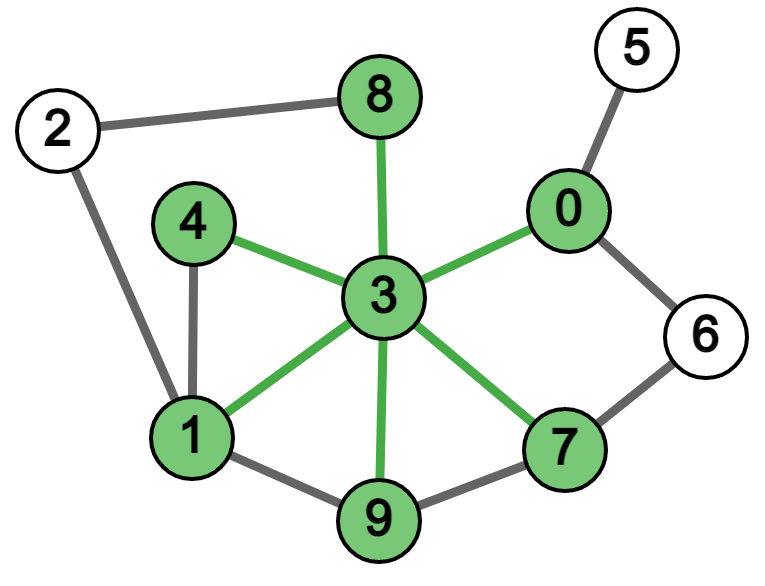
\includegraphics[scale=.25]{img/ego_3.png}
  \caption{3's ego includes $0,1,3,4,7,8,9$ and all edges between them.}
  \label{fig:core_ex}
\end{figure}

The ego $G_x$ of a vertex $x$ from a network $N=(V,E)$ is the set $V(G_x)$ (vertices of the $G_x$)
of all vertices that have an edge with it, as well as all the edges with vertices in $V(G_x)$.

Formally, for
$V(G_x) \subset V$ and $E(G_x) \subset E$:

$$E(G_x)=\{e : v_e,u_e \in H_x\}$$

In the library, the algorithm takes in a vertex's ID, and returns a Network instance.
\begin{minted}[bgcolor=bg]{ts}
ego(id: base_id): Network {
  const ego_network = new Network(this.args);

  this.edges.forEach((edge) => {
    const { from, to } = edge.vertices;
    if (from === id || to === id) {
      ego_network.addEdge({ from, to });
    }
  });

  this.edges.forEach(({ vertices }) => {
    const { from, to } = vertices;
    if (ego_network.vertices.has(from) &&
        ego_network.vertices.has(to))
      ego_network.addEdge({ from, to });
  });

  return ego_network;
}
\end{minted}

First, the algorithm goes through all edges, and add to the \mintinline{ts}{ego_network}
the ones that contain the given vertex.
Then, it goes through the edges of the network again,
this time adding edges that don't connect to the ego vertex,
but connect to vertices already in the ego network.

\section{Copy}

It is very useful to have a copy of a network
when we want another network that derives from it.
For example, a core-decomposition (as we will see next)
makes use of the copy function.

Because of the way JS works, making a copy of a class' instance
is not as simple as:
\begin{minted}[bgcolor=bg]{ts}
const net_copy = net;
\end{minted}

This method works more like a reference to the original object.
If a property of net changes, \mintinline{ts}{net_copy} will also change.

Nevertheless, there are many other ways of making copies of objects with JS.
Here are some of the most common:
\begin{minted}[bgcolor=bg]{ts}
// Destructuring:
const copy_destructure = { ...net }

// Assign:
const copy_assign = Object.assign({}, net)

// JSON:
const copy_json = JSON.parse(JSON.stringify(net))
\end{minted}

However, none of these suit our need for a completely independent copy.
For destructuring, although simple properties such as the maximum number of edges of the Network would be properly copied,
objects (which are most of the network) would still become references.
Assigning has the same issue.
The edges property, for instance, would become a reference because it is a Map.
So if an edge is added to the original, the copy would also receive it.

The JSON method solves this problem.
It transforms the network into a JSON string, and then transforms it back into an object with \mintinline{ts}{JSON.parse}.
The big problem with this is that the copy is no longer a network instance, just an object with many of the properties a network would have.
This is an issue we would want to avoid even more when we consider typing and interfaces are precisely why TS was chosen.

Thus, the copy algorithm works differently, and is specific to the Network class:

\begin{minted}[bgcolor=bg]{ts}
copy(): Network {
  const network_copy = new Network(this.args);
  network_copy.addEdgeMap(this.edges);
  network_copy.addVertexMap(this.vertices);
  return network_copy;
}
\end{minted}

\section{Core}

A k-core decomposition of a network $N$ is a subgraph $C_k$ with any
$v\in V(N)$ with $D_v<k$ removed recursively.
This means, we remove all vertices with degree less than $k$,
then in the resulting network, we remove all vertices with
degree less than $k$, and so on until there are no vertices
where $D_v<k$.
$$C_k=(V_c,E_c)$$
$$V_c=\{v:v\in V(N),D_v\geq k\}, E_c=\{e:e\in E(N)\}$$
The core function only ends after all vertices with degree less than $k$ are removed.
It returns a network class instance.

\begin{minted}[bgcolor=bg]{ts}
core(k: number): Network {
  const k_decomposition = this.copy();

  while (k > 0 && k_decomposition.vertices.size > 0) {
    let { vertex_list } = k_decomposition;
    let vertex_counter;
    for (
      vertex_counter = 0;
      vertex_counter < vertex_list.length;
      vertex_counter++
    ) {
      const current_vertex =
        k_decomposition.vertex_list[vertex_counter];
      if (k_decomposition.degree(current_vertex.id) < k) {
        k_decomposition.removeVertex(current_vertex.id);
        vertex_list = k_decomposition.vertex_list;
        vertex_counter = 0;
      }
    }
    k--;
  }

  return k_decomposition;
}
\end{minted}

\begin{figure}[H]
  \centering
  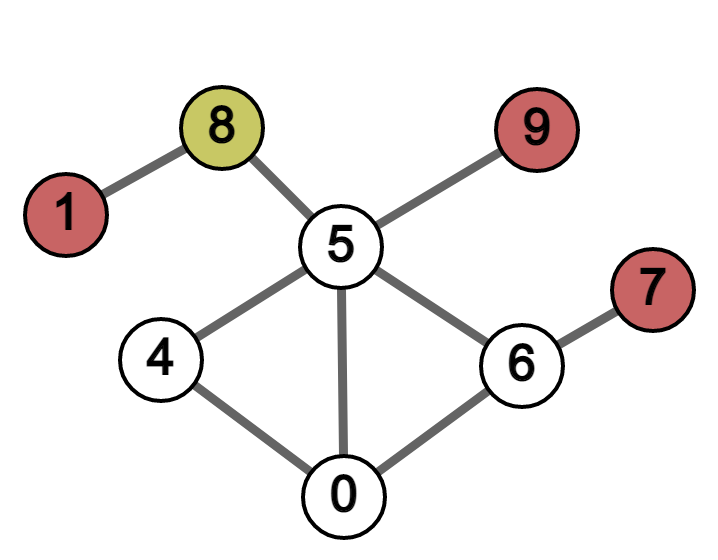
\includegraphics[scale=.25]{img/core_ex.png}
  \caption{A 2-core decomposition would remove nodes $1,9,7,8$. $8$ would be removed in the second iteration of the function.}
  \label{fig:core_ex}
\end{figure}


\section{Clustering}

The clustering coefficient measures how connected the neighbors of a vertex are to each other.
It is the number of edges that exist in between the vertex's neighbors in relation to the
maximum number of edges that could exist there.

$$\frac{|\{e:v,u\in e \wedge v,u\in H[x]\}|}{|H[x]|(|H[x]|-1)}$$

\begin{minted}[bgcolor=bg]{ts}
clustering(id: base_id): number {
  const ego_net = this.ego(id);

  if (ego_net.vertices.size <= 1) return 0;

  const centerless_ego = ego_net;

  // Max edges in a network without the given vertex.
  centerless_ego.removeVertex(id);
  const { max_edges } = centerless_ego;
  const existing_edges = centerless_ego.edges.size;

  // If graph is directed, multiply result by 2.
  const directed_const = this.is_directed ? 2 : 1;

  return directed_const * (existing_edges / max_edges);
}
\end{minted}

The algorithm makes use of the \mintinline{ts}{ego} function, removing the ID vertex after.
It also uses a tenary operator because the only difference between the clustering
from a directed network to an undirected one is
that the former has its clustering multiplied by 2.

\section{Average Clustering}

This function calculates the average clustering of the network.
If calculates the clustering coefficient of all vertices, inserting its values into an array.
It then reduces the array, summing all of its values.
Finally, it returns the average, which devides the sum by the number of vertices in the network.
\begin{minted}[bgcolor=bg]{ts}
averageClustering(): number {
  let average_clustering = 0;

  if (this.vertices.size <= 1) return average_clustering;

  const clustering_sum = this.vertex_list
    .map((vertex) => this.clustering(vertex.id))
    .reduce((prev, curr) => prev + curr);

  average_clustering = clustering_sum / this.vertices.size;

  return average_clustering;
}
\end{minted}

\section{Triplets}

A triplet is a set of 3 vertices and 3 edges connecting said vertices.
Triplets, also called triangles, triples or $K_3$s,
are the foundation of design theory,
an entrire field of mathematics.
Design theory is concerned with decomposing graphs into triplets.

\begin{figure}[H]
  \centering
  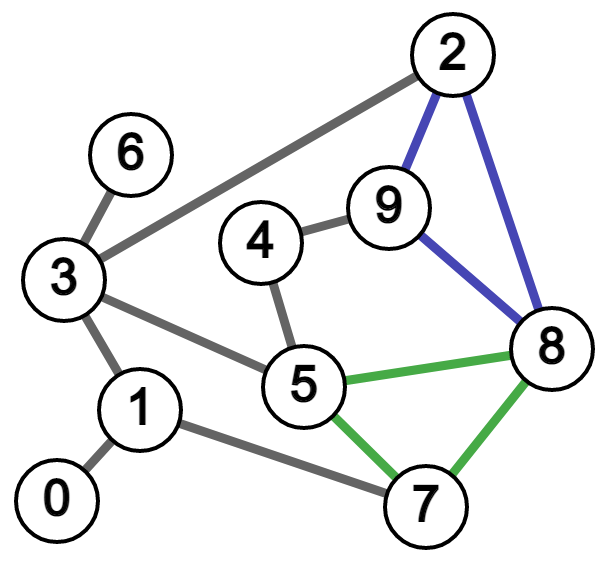
\includegraphics[scale=.25]{img/triplets.png}
  \caption{This network has two triplets: $\{5,7,8\}$ and $\{2,8,9\}$.}
  \label{fig:core_ex}
\end{figure}
The triplets algorithm in NeTS went through many iterations that improved its performance.
The first algorithm looked through all edges, and, while in each edge,
looked through all nodes and checked for any that had edges with the two nodes in the edge.
The most glaring problem with this is that it counts each triplet three times:
once for each edge.

The solution was to order the triplets so that, internally, the algorithm
sees $5,8,7$ as different from $5,7,8$, for example.
This was initially done by comparing the triplet that could be created
with the sorted version of that triplet.
The improved version only needs to check if the current vertices are already sorted:
\begin{minted}[bgcolor=bg]{ts}
k2.isSameTriplet(triplet, triplet.sort())
\end{minted}

The current iteration of the triplets algorithm also does not go through all vertices in the network.
It only looks through the neighbors of one of the vertices in the edge being analysed.
This also saves us from having to check if both vertices have edges with the vertice beeing looked at.

\begin{minted}[bgcolor=bg]{ts}
triplets(): Triplet[] {
  const triplet_list: Triplet[] = [];

  const k2 = this.core(2);

  const { vertices, edges } = k2;

  edges.forEach((edge) => {
    const { from, to } = edge.vertices;
    k2.neighbors(from).forEach((id) => {
      if (edge.hasVertex(id)) return;
      const triplet: Triplet = [id, ...[from, to].sort()];
      if (k2.isSameTriplet(triplet, triplet.sort()))
        if (k2.hasEdge(id, to, true))
          triplet_list.push(triplet);
    });
  });

  return triplet_list;
}
\end{minted}
